\subsection{Posterior-Mean Interval Comparisons}
\label{sec:supp-mti-full-validation}

The additional Gibbs comparison uses the same 72,000 simulation datasets
as the calibrated three-method comparison. For each dataset,
\(I_{\mathrm G}\) uses the posterior-mean endpoints at its recorded
ECM-selected \(q,\delta\). The empirical content-attainment proportion
and the raw width distribution therefore describe a separately specified
endpoint summary at the same selected target. The DP content check and
calibrated ECM rule remain unchanged.

Across the 72 settings, posterior-mean interval attainment ranges from
\MTIFullAttainmentMin\% to \MTIFullAttainmentMax\%.
Exact binomial intervals adjusted over the 72 settings for this method
have lower bounds above 0.95 in every setting; the smallest lower bound
is \MTIFullSimultaneousLower{}. Each tail uses probability
\(0.05/(2\cdot72)\). These statements quantify Monte Carlo uncertainty
over the specified simulation panel. They provide empirical evidence for
these distributions and settings, with the general tolerance question
retaining the assumptions and limitations stated above.

Mean Gibbs width is greater than ECM and Young--Mathew mean width in
every setting; it is smaller than Wilks mean width in
\MTIFullShorterWilks{} settings. At \(n=1000,c=0.90\), Normal mean widths
are \MTIFullNormalECM{} for ECM and \MTIFullNormalGibbs{} for Gibbs,
whereas Gamma mean widths are \MTIFullGammaECM{} and
\MTIFullGammaGibbs{}, respectively. In that Gamma setting, every selected
tilt is empirically limiting. Outward lower-endpoint dispersion accounts
for most of the extra width. Thus a large sample can yield a precise
Monte Carlo calculation of a broad posterior under the specified prior.

The endpoint-median sensitivity summary has attainment between
\MTIFullMedianAttainmentMin\% and \MTIFullMedianAttainmentMax\%, and its
mean width also exceeds ECM mean width in all 72 settings. That comparison
uses the difference of the two endpoint medians. The posterior median of
width is a different quantity, recorded with its own credible interval.

Figure~\ref{fig:supp-mti-full-attainment} summarizes the content-attainment
range across distributions for each design. Table~\ref{tab:supp-mti-full-simulation}
and the following distribution-specific tables give all four methods'
attainment and raw width ranges. The width figures retain individual
distribution/design summaries, without averaging lengths across laws.

\begin{figure}[p]
\centering
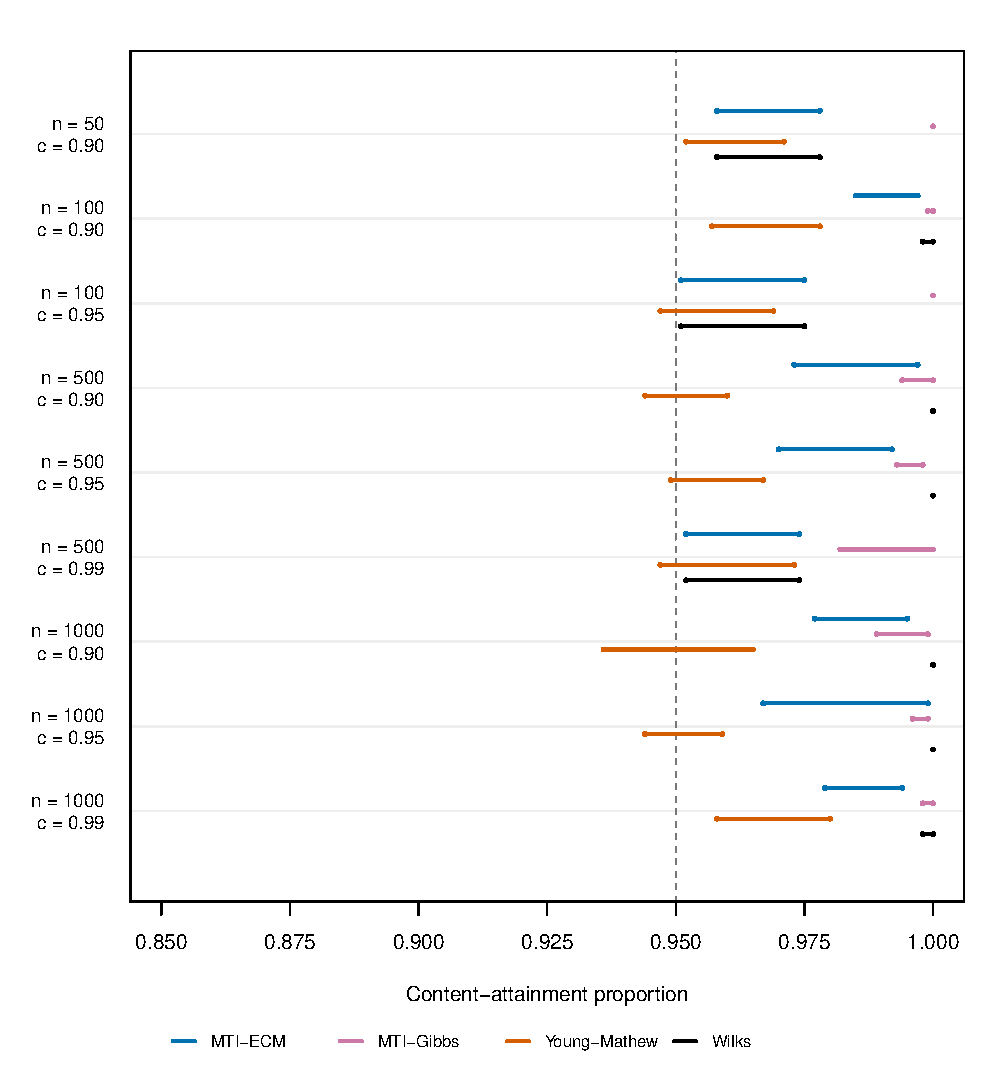
\includegraphics[width=\textwidth]{figures/generated/figS_mti_full_attainment.pdf}
\caption{\textbf{Content attainment including posterior-mean intervals.}
Each horizontal segment spans the observed attainment proportions across
the eight simulation distributions for one design and method. These
segments describe distributional variation; binomial Monte Carlo bounds
are recorded separately. The dashed line marks tolerance confidence
0.95. MTI-Gibbs uses the fixed-target posterior-mean endpoints defined
above.}
\label{fig:supp-mti-full-attainment}
\end{figure}

\begingroup
\footnotesize
\setlength{\tabcolsep}{4pt}
\renewcommand{\arraystretch}{1.06}
\clearpage
\begin{longtable}{@{}rrlrr@{}}
\caption{\textbf{Normal: paired interval comparison.} Each design uses 1000 independent samples at tolerance confidence 0.95. Attainment is the percentage with true population content at least \(c\). Width ranges are empirical 2.5\%--97.5\% quantiles across those samples. MTI-Gibbs uses posterior-mean endpoints at the ECM-selected fitted content and tilt.}\label{tab:supp-mti-full-simulation}\\
\toprule
\(n\) & \(c\) & Method & Attainment (\%) & Width range\\
\midrule
\endfirsthead
\caption[]{Normal: paired interval comparison (continued).}\\
\toprule
\(n\) & \(c\) & Method & Attainment (\%) & Width range\\
\midrule
\endhead
\bottomrule
\endfoot
50 & 0.90 & MTI-ECM & 97.1 & 3.406--5.810 \\
 &  & MTI-Gibbs & 100.0 & 6.099--7.696 \\
 &  & Young--Mathew & 96.6 & 3.333--5.568 \\
 &  & Wilks & 97.1 & 3.406--5.810 \\
\addlinespace[0.3em]
100 & 0.90 & MTI-ECM & 98.6 & 3.438--4.622 \\
 &  & MTI-Gibbs & 100.0 & 3.875--80.261 \\
 &  & Young--Mathew & 97.2 & 3.362--4.845 \\
 &  & Wilks & 100.0 & 3.947--6.389 \\
\addlinespace[0.3em]
100 & 0.95 & MTI-ECM & 97.5 & 4.037--6.331 \\
 &  & MTI-Gibbs & 100.0 & 5.255--7.099 \\
 &  & Young--Mathew & 96.7 & 3.995--6.172 \\
 &  & Wilks & 97.5 & 4.037--6.331 \\
\addlinespace[0.3em]
500 & 0.90 & MTI-ECM & 97.3 & 3.308--3.854 \\
 &  & MTI-Gibbs & 99.4 & 3.398--3.949 \\
 &  & Young--Mathew & 95.8 & 3.263--3.826 \\
 &  & Wilks & 100.0 & 5.195--7.201 \\
\addlinespace[0.3em]
500 & 0.95 & MTI-ECM & 97.0 & 3.945--4.690 \\
 &  & MTI-Gibbs & 99.7 & 4.103--4.883 \\
 &  & Young--Mathew & 96.6 & 3.902--4.693 \\
 &  & Wilks & 100.0 & 5.200--7.271 \\
\addlinespace[0.3em]
500 & 0.99 & MTI-ECM & 96.5 & 5.218--7.204 \\
 &  & MTI-Gibbs & 100.0 & 5.858--7.503 \\
 &  & Young--Mathew & 96.5 & 5.192--7.076 \\
 &  & Wilks & 96.5 & 5.218--7.204 \\
\addlinespace[0.3em]
1000 & 0.90 & MTI-ECM & 97.7 & 3.307--3.669 \\
 &  & MTI-Gibbs & 99.5 & 3.360--3.721 \\
 &  & Young--Mathew & 96.2 & 3.265--3.641 \\
 &  & Wilks & 100.0 & 5.594--7.618 \\
\addlinespace[0.3em]
1000 & 0.95 & MTI-ECM & 96.7 & 3.927--4.418 \\
 &  & MTI-Gibbs & 99.6 & 3.999--4.503 \\
 &  & Young--Mathew & 95.3 & 3.901--4.406 \\
 &  & Wilks & 100.0 & 5.642--7.561 \\
\addlinespace[0.3em]
1000 & 0.99 & MTI-ECM & 97.9 & 5.261--6.437 \\
 &  & MTI-Gibbs & 99.9 & 5.602--82.482 \\
 &  & Young--Mathew & 98.0 & 5.246--6.410 \\
 &  & Wilks & 99.9 & 5.636--7.633 \\
\addlinespace[0.3em]
\end{longtable}
\clearpage
\begin{longtable}{@{}rrlrr@{}}
\caption{\textbf{Student t (3 df): paired interval comparison.} Each design uses 1000 independent samples at tolerance confidence 0.95. Attainment is the percentage with true population content at least \(c\). Width ranges are empirical 2.5\%--97.5\% quantiles across those samples. MTI-Gibbs uses posterior-mean endpoints at the ECM-selected fitted content and tilt.}\label{tab:supp-mti-full-student_t3}\\
\toprule
\(n\) & \(c\) & Method & Attainment (\%) & Width range\\
\midrule
\endfirsthead
\caption[]{Student t (3 df): paired interval comparison (continued).}\\
\toprule
\(n\) & \(c\) & Method & Attainment (\%) & Width range\\
\midrule
\endhead
\bottomrule
\endfoot
50 & 0.90 & MTI-ECM & 95.8 & 2.815--12.250 \\
 &  & MTI-Gibbs & 100.0 & 5.872--164.895 \\
 &  & Young--Mathew & 95.2 & 2.741--10.704 \\
 &  & Wilks & 95.8 & 2.815--12.250 \\
\addlinespace[0.3em]
100 & 0.90 & MTI-ECM & 98.5 & 3.034--5.722 \\
 &  & MTI-Gibbs & 100.0 & 3.757--82.039 \\
 &  & Young--Mathew & 97.8 & 2.901--6.808 \\
 &  & Wilks & 100.0 & 3.674--17.480 \\
\addlinespace[0.3em]
100 & 0.95 & MTI-ECM & 96.8 & 3.829--16.167 \\
 &  & MTI-Gibbs & 100.0 & 5.095--17.146 \\
 &  & Young--Mathew & 96.1 & 3.774--14.599 \\
 &  & Wilks & 96.8 & 3.829--16.167 \\
\addlinespace[0.3em]
500 & 0.90 & MTI-ECM & 97.6 & 2.763--3.591 \\
 &  & MTI-Gibbs & 99.7 & 2.879--3.722 \\
 &  & Young--Mathew & 95.4 & 2.700--3.537 \\
 &  & Wilks & 100.0 & 7.078--25.555 \\
\addlinespace[0.3em]
500 & 0.95 & MTI-ECM & 97.8 & 3.745--5.446 \\
 &  & MTI-Gibbs & 99.4 & 3.993--5.978 \\
 &  & Young--Mathew & 96.7 & 3.701--5.405 \\
 &  & Wilks & 100.0 & 7.037--26.491 \\
\addlinespace[0.3em]
500 & 0.99 & MTI-ECM & 95.5 & 6.910--27.512 \\
 &  & MTI-Gibbs & 98.2 & 7.341--34.019 \\
 &  & Young--Mathew & 95.3 & 6.818--26.038 \\
 &  & Wilks & 95.5 & 6.910--27.512 \\
\addlinespace[0.3em]
1000 & 0.90 & MTI-ECM & 97.9 & 2.762--3.278 \\
 &  & MTI-Gibbs & 99.5 & 2.830--3.350 \\
 &  & Young--Mathew & 96.5 & 2.706--3.226 \\
 &  & Wilks & 100.0 & 8.730--33.802 \\
\addlinespace[0.3em]
1000 & 0.95 & MTI-ECM & 98.2 & 3.741--4.729 \\
 &  & MTI-Gibbs & 99.6 & 3.859--4.929 \\
 &  & Young--Mathew & 95.9 & 3.645--4.690 \\
 &  & Wilks & 100.0 & 8.790--32.532 \\
\addlinespace[0.3em]
1000 & 0.99 & MTI-ECM & 98.8 & 7.129--12.377 \\
 &  & MTI-Gibbs & 99.8 & 8.488--88.833 \\
 &  & Young--Mathew & 97.2 & 7.022--14.800 \\
 &  & Wilks & 99.8 & 8.828--33.768 \\
\addlinespace[0.3em]
\end{longtable}
\clearpage
\begin{longtable}{@{}rrlrr@{}}
\caption{\textbf{Exponential: paired interval comparison.} Each design uses 1000 independent samples at tolerance confidence 0.95. Attainment is the percentage with true population content at least \(c\). Width ranges are empirical 2.5\%--97.5\% quantiles across those samples. MTI-Gibbs uses posterior-mean endpoints at the ECM-selected fitted content and tilt.}\label{tab:supp-mti-full-exponential}\\
\toprule
\(n\) & \(c\) & Method & Attainment (\%) & Width range\\
\midrule
\endfirsthead
\caption[]{Exponential: paired interval comparison (continued).}\\
\toprule
\(n\) & \(c\) & Method & Attainment (\%) & Width range\\
\midrule
\endhead
\bottomrule
\endfoot
50 & 0.90 & MTI-ECM & 97.4 & 2.685--7.534 \\
 &  & MTI-Gibbs & 100.0 & 6.262--85.616 \\
 &  & Young--Mathew & 96.8 & 2.622--6.931 \\
 &  & Wilks & 97.4 & 2.685--7.534 \\
\addlinespace[0.3em]
100 & 0.90 & MTI-ECM & 99.0 & 2.657--4.756 \\
 &  & MTI-Gibbs & 100.0 & 4.539--81.740 \\
 &  & Young--Mathew & 95.7 & 2.903--6.123 \\
 &  & Wilks & 100.0 & 3.305--8.567 \\
\addlinespace[0.3em]
100 & 0.95 & MTI-ECM & 95.2 & 3.250--8.068 \\
 &  & MTI-Gibbs & 100.0 & 5.135--118.585 \\
 &  & Young--Mathew & 94.9 & 3.213--7.576 \\
 &  & Wilks & 95.2 & 3.250--8.068 \\
\addlinespace[0.3em]
500 & 0.90 & MTI-ECM & 99.3 & 2.402--3.026 \\
 &  & MTI-Gibbs & 99.8 & 2.993--73.266 \\
 &  & Young--Mathew & 95.1 & 2.819--3.751 \\
 &  & Wilks & 100.0 & 4.870--10.021 \\
\addlinespace[0.3em]
500 & 0.95 & MTI-ECM & 99.0 & 3.131--4.152 \\
 &  & MTI-Gibbs & 99.5 & 4.059--78.594 \\
 &  & Young--Mathew & 96.3 & 3.560--5.035 \\
 &  & Wilks & 100.0 & 4.985--10.122 \\
\addlinespace[0.3em]
500 & 0.99 & MTI-ECM & 97.1 & 5.012--9.520 \\
 &  & MTI-Gibbs & 100.0 & 6.812--58.762 \\
 &  & Young--Mathew & 96.8 & 4.983--9.125 \\
 &  & Wilks & 97.1 & 5.012--9.520 \\
\addlinespace[0.3em]
1000 & 0.90 & MTI-ECM & 98.8 & 2.366--2.782 \\
 &  & MTI-Gibbs & 99.5 & 2.889--69.788 \\
 &  & Young--Mathew & 93.6 & 2.863--3.458 \\
 &  & Wilks & 100.0 & 5.612--10.662 \\
\addlinespace[0.3em]
1000 & 0.95 & MTI-ECM & 99.5 & 3.097--3.798 \\
 &  & MTI-Gibbs & 99.7 & 3.812--74.197 \\
 &  & Young--Mathew & 94.9 & 3.530--4.445 \\
 &  & Wilks & 100.0 & 5.548--10.262 \\
\addlinespace[0.3em]
1000 & 0.99 & MTI-ECM & 99.3 & 4.963--7.395 \\
 &  & MTI-Gibbs & 100.0 & 52.407--85.792 \\
 &  & Young--Mathew & 95.9 & 5.190--8.262 \\
 &  & Wilks & 99.9 & 5.542--10.583 \\
\addlinespace[0.3em]
\end{longtable}
\clearpage
\begin{longtable}{@{}rrlrr@{}}
\caption{\textbf{Asymmetric Laplace: paired interval comparison.} Each design uses 1000 independent samples at tolerance confidence 0.95. Attainment is the percentage with true population content at least \(c\). Width ranges are empirical 2.5\%--97.5\% quantiles across those samples. MTI-Gibbs uses posterior-mean endpoints at the ECM-selected fitted content and tilt.}\label{tab:supp-mti-full-asym_laplace_tau010}\\
\toprule
\(n\) & \(c\) & Method & Attainment (\%) & Width range\\
\midrule
\endfirsthead
\caption[]{Asymmetric Laplace: paired interval comparison (continued).}\\
\toprule
\(n\) & \(c\) & Method & Attainment (\%) & Width range\\
\midrule
\endhead
\bottomrule
\endfoot
50 & 0.90 & MTI-ECM & 96.9 & 2.710--7.197 \\
 &  & MTI-Gibbs & 100.0 & 6.079--80.116 \\
 &  & Young--Mathew & 95.9 & 2.651--6.643 \\
 &  & Wilks & 96.9 & 2.710--7.197 \\
\addlinespace[0.3em]
100 & 0.90 & MTI-ECM & 99.4 & 2.853--4.778 \\
 &  & MTI-Gibbs & 100.0 & 3.724--81.686 \\
 &  & Young--Mathew & 97.0 & 2.982--6.137 \\
 &  & Wilks & 100.0 & 3.584--8.326 \\
\addlinespace[0.3em]
100 & 0.95 & MTI-ECM & 97.4 & 3.575--8.497 \\
 &  & MTI-Gibbs & 100.0 & 5.186--113.330 \\
 &  & Young--Mathew & 96.9 & 3.530--8.070 \\
 &  & Wilks & 97.4 & 3.575--8.497 \\
\addlinespace[0.3em]
500 & 0.90 & MTI-ECM & 98.8 & 2.588--3.284 \\
 &  & MTI-Gibbs & 99.9 & 2.741--69.324 \\
 &  & Young--Mathew & 95.3 & 2.859--3.729 \\
 &  & Wilks & 100.0 & 5.230--10.463 \\
\addlinespace[0.3em]
500 & 0.95 & MTI-ECM & 97.9 & 3.374--4.476 \\
 &  & MTI-Gibbs & 99.6 & 3.632--78.520 \\
 &  & Young--Mathew & 95.8 & 3.591--5.114 \\
 &  & Wilks & 100.0 & 5.223--10.259 \\
\addlinespace[0.3em]
500 & 0.99 & MTI-ECM & 97.4 & 5.294--10.272 \\
 &  & MTI-Gibbs & 100.0 & 6.682--60.873 \\
 &  & Young--Mathew & 97.1 & 5.262--9.865 \\
 &  & Wilks & 97.4 & 5.294--10.272 \\
\addlinespace[0.3em]
1000 & 0.90 & MTI-ECM & 98.9 & 2.587--3.052 \\
 &  & MTI-Gibbs & 99.8 & 2.660--3.161 \\
 &  & Young--Mathew & 96.3 & 2.863--3.452 \\
 &  & Wilks & 100.0 & 5.987--11.268 \\
\addlinespace[0.3em]
1000 & 0.95 & MTI-ECM & 97.9 & 3.359--4.059 \\
 &  & MTI-Gibbs & 99.8 & 3.495--71.517 \\
 &  & Young--Mathew & 95.3 & 3.572--4.503 \\
 &  & Wilks & 100.0 & 5.974--11.303 \\
\addlinespace[0.3em]
1000 & 0.99 & MTI-ECM & 99.1 & 5.376--7.828 \\
 &  & MTI-Gibbs & 100.0 & 6.413--86.209 \\
 &  & Young--Mathew & 97.1 & 5.473--8.591 \\
 &  & Wilks & 99.9 & 6.065--11.441 \\
\addlinespace[0.3em]
\end{longtable}
\clearpage
\begin{longtable}{@{}rrlrr@{}}
\caption{\textbf{Two-piece Normal: paired interval comparison.} Each design uses 1000 independent samples at tolerance confidence 0.95. Attainment is the percentage with true population content at least \(c\). Width ranges are empirical 2.5\%--97.5\% quantiles across those samples. MTI-Gibbs uses posterior-mean endpoints at the ECM-selected fitted content and tilt.}\label{tab:supp-mti-full-two_piece_normal_1_12}\\
\toprule
\(n\) & \(c\) & Method & Attainment (\%) & Width range\\
\midrule
\endfirsthead
\caption[]{Two-piece Normal: paired interval comparison (continued).}\\
\toprule
\(n\) & \(c\) & Method & Attainment (\%) & Width range\\
\midrule
\endhead
\bottomrule
\endfoot
50 & 0.90 & MTI-ECM & 96.1 & 2.993--5.780 \\
 &  & MTI-Gibbs & 100.0 & 6.040--62.283 \\
 &  & Young--Mathew & 95.2 & 2.946--5.471 \\
 &  & Wilks & 96.1 & 2.993--5.780 \\
\addlinespace[0.3em]
100 & 0.90 & MTI-ECM & 98.9 & 3.052--4.348 \\
 &  & MTI-Gibbs & 100.0 & 3.840--79.737 \\
 &  & Young--Mathew & 96.5 & 3.141--4.966 \\
 &  & Wilks & 99.8 & 3.545--6.144 \\
\addlinespace[0.3em]
100 & 0.95 & MTI-ECM & 95.1 & 3.508--6.118 \\
 &  & MTI-Gibbs & 100.0 & 5.039--7.420 \\
 &  & Young--Mathew & 94.7 & 3.482--5.853 \\
 &  & Wilks & 95.1 & 3.508--6.118 \\
\addlinespace[0.3em]
500 & 0.90 & MTI-ECM & 98.5 & 2.910--3.394 \\
 &  & MTI-Gibbs & 99.5 & 3.026--70.269 \\
 &  & Young--Mathew & 94.4 & 3.098--3.679 \\
 &  & Wilks & 100.0 & 4.575--6.808 \\
\addlinespace[0.3em]
500 & 0.95 & MTI-ECM & 98.5 & 3.462--4.150 \\
 &  & MTI-Gibbs & 99.8 & 3.691--76.960 \\
 &  & Young--Mathew & 94.9 & 3.630--4.443 \\
 &  & Wilks & 100.0 & 4.577--6.806 \\
\addlinespace[0.3em]
500 & 0.99 & MTI-ECM & 96.9 & 4.560--6.751 \\
 &  & MTI-Gibbs & 100.0 & 5.776--7.988 \\
 &  & Young--Mathew & 96.4 & 4.543--6.563 \\
 &  & Wilks & 96.9 & 4.560--6.751 \\
\addlinespace[0.3em]
1000 & 0.90 & MTI-ECM & 98.0 & 2.879--3.216 \\
 &  & MTI-Gibbs & 99.5 & 2.949--3.459 \\
 &  & Young--Mathew & 94.9 & 3.099--3.491 \\
 &  & Wilks & 100.0 & 4.971--7.137 \\
\addlinespace[0.3em]
1000 & 0.95 & MTI-ECM & 98.7 & 3.446--3.892 \\
 &  & MTI-Gibbs & 99.9 & 3.566--70.388 \\
 &  & Young--Mathew & 95.4 & 3.606--4.159 \\
 &  & Wilks & 100.0 & 4.965--7.246 \\
\addlinespace[0.3em]
1000 & 0.99 & MTI-ECM & 98.9 & 4.629--5.807 \\
 &  & MTI-Gibbs & 99.8 & 5.243--83.205 \\
 &  & Young--Mathew & 96.1 & 4.686--6.170 \\
 &  & Wilks & 99.9 & 5.000--6.978 \\
\addlinespace[0.3em]
\end{longtable}
\clearpage
\begin{longtable}{@{}rrlrr@{}}
\caption{\textbf{Beta(1,8): paired interval comparison.} Each design uses 1000 independent samples at tolerance confidence 0.95. Attainment is the percentage with true population content at least \(c\). Width ranges are empirical 2.5\%--97.5\% quantiles across those samples. MTI-Gibbs uses posterior-mean endpoints at the ECM-selected fitted content and tilt.}\label{tab:supp-mti-full-beta18}\\
\toprule
\(n\) & \(c\) & Method & Attainment (\%) & Width range\\
\midrule
\endfirsthead
\caption[]{Beta(1,8): paired interval comparison (continued).}\\
\toprule
\(n\) & \(c\) & Method & Attainment (\%) & Width range\\
\midrule
\endhead
\bottomrule
\endfoot
50 & 0.90 & MTI-ECM & 97.8 & 2.798--6.097 \\
 &  & MTI-Gibbs & 100.0 & 6.195--67.772 \\
 &  & Young--Mathew & 97.1 & 2.754--5.753 \\
 &  & Wilks & 97.8 & 2.798--6.097 \\
\addlinespace[0.3em]
100 & 0.90 & MTI-ECM & 99.1 & 2.861--4.477 \\
 &  & MTI-Gibbs & 100.0 & 4.207--79.951 \\
 &  & Young--Mathew & 95.7 & 3.064--5.182 \\
 &  & Wilks & 100.0 & 3.468--6.465 \\
\addlinespace[0.3em]
100 & 0.95 & MTI-ECM & 96.9 & 3.351--6.285 \\
 &  & MTI-Gibbs & 100.0 & 5.130--7.806 \\
 &  & Young--Mathew & 96.1 & 3.309--6.046 \\
 &  & Wilks & 96.9 & 3.351--6.285 \\
\addlinespace[0.3em]
500 & 0.90 & MTI-ECM & 99.0 & 2.593--3.166 \\
 &  & MTI-Gibbs & 99.6 & 3.097--72.436 \\
 &  & Young--Mathew & 96.0 & 2.999--3.733 \\
 &  & Wilks & 100.0 & 4.642--7.116 \\
\addlinespace[0.3em]
500 & 0.95 & MTI-ECM & 98.1 & 3.202--4.100 \\
 &  & MTI-Gibbs & 99.4 & 3.981--77.669 \\
 &  & Young--Mathew & 94.9 & 3.592--4.639 \\
 &  & Wilks & 100.0 & 4.540--7.131 \\
\addlinespace[0.3em]
500 & 0.99 & MTI-ECM & 95.2 & 4.551--7.141 \\
 &  & MTI-Gibbs & 100.0 & 6.263--8.836 \\
 &  & Young--Mathew & 94.8 & 4.535--6.978 \\
 &  & Wilks & 95.2 & 4.551--7.141 \\
\addlinespace[0.3em]
1000 & 0.90 & MTI-ECM & 99.2 & 2.576--2.970 \\
 &  & MTI-Gibbs & 99.7 & 2.988--68.655 \\
 &  & Young--Mathew & 94.7 & 3.002--3.485 \\
 &  & Wilks & 100.0 & 5.088--7.341 \\
\addlinespace[0.3em]
1000 & 0.95 & MTI-ECM & 99.2 & 3.207--3.769 \\
 &  & MTI-Gibbs & 99.8 & 3.727--73.365 \\
 &  & Young--Mathew & 94.4 & 3.582--4.276 \\
 &  & Wilks & 100.0 & 5.077--7.388 \\
\addlinespace[0.3em]
1000 & 0.99 & MTI-ECM & 98.7 & 4.621--6.028 \\
 &  & MTI-Gibbs & 100.0 & 49.957--83.735 \\
 &  & Young--Mathew & 96.0 & 4.787--6.407 \\
 &  & Wilks & 100.0 & 5.105--7.393 \\
\addlinespace[0.3em]
\end{longtable}
\clearpage
\begin{longtable}{@{}rrlrr@{}}
\caption{\textbf{Gamma(0.5,1): paired interval comparison.} Each design uses 1000 independent samples at tolerance confidence 0.95. Attainment is the percentage with true population content at least \(c\). Width ranges are empirical 2.5\%--97.5\% quantiles across those samples. MTI-Gibbs uses posterior-mean endpoints at the ECM-selected fitted content and tilt.}\label{tab:supp-mti-full-gamma05}\\
\toprule
\(n\) & \(c\) & Method & Attainment (\%) & Width range\\
\midrule
\endfirsthead
\caption[]{Gamma(0.5,1): paired interval comparison (continued).}\\
\toprule
\(n\) & \(c\) & Method & Attainment (\%) & Width range\\
\midrule
\endhead
\bottomrule
\endfoot
50 & 0.90 & MTI-ECM & 97.6 & 2.373--8.494 \\
 &  & MTI-Gibbs & 100.0 & 6.845--101.841 \\
 &  & Young--Mathew & 97.0 & 2.333--7.750 \\
 &  & Wilks & 97.6 & 2.373--8.494 \\
\addlinespace[0.3em]
100 & 0.90 & MTI-ECM & 99.7 & 2.393--4.902 \\
 &  & MTI-Gibbs & 99.9 & 45.023--81.451 \\
 &  & Young--Mathew & 95.7 & 2.679--6.430 \\
 &  & Wilks & 99.9 & 3.120--9.220 \\
\addlinespace[0.3em]
100 & 0.95 & MTI-ECM & 96.2 & 3.188--9.257 \\
 &  & MTI-Gibbs & 100.0 & 5.538--153.714 \\
 &  & Young--Mathew & 95.6 & 3.153--8.634 \\
 &  & Wilks & 96.2 & 3.188--9.257 \\
\addlinespace[0.3em]
500 & 0.90 & MTI-ECM & 99.7 & 2.034--2.768 \\
 &  & MTI-Gibbs & 100.0 & 43.106--73.456 \\
 &  & Young--Mathew & 94.5 & 2.574--3.632 \\
 &  & Wilks & 100.0 & 5.086--11.245 \\
\addlinespace[0.3em]
500 & 0.95 & MTI-ECM & 98.7 & 2.849--4.141 \\
 &  & MTI-Gibbs & 99.3 & 44.039--78.670 \\
 &  & Young--Mathew & 95.3 & 3.383--5.200 \\
 &  & Wilks & 100.0 & 5.221--11.450 \\
\addlinespace[0.3em]
500 & 0.99 & MTI-ECM & 97.4 & 5.199--12.000 \\
 &  & MTI-Gibbs & 99.9 & 7.867--67.419 \\
 &  & Young--Mathew & 97.3 & 5.142--11.244 \\
 &  & Wilks & 97.4 & 5.199--12.000 \\
\addlinespace[0.3em]
1000 & 0.90 & MTI-ECM & 98.8 & 1.971--2.489 \\
 &  & MTI-Gibbs & 98.9 & 44.535--69.312 \\
 &  & Young--Mathew & 95.7 & 2.587--3.286 \\
 &  & Wilks & 100.0 & 5.965--11.997 \\
\addlinespace[0.3em]
1000 & 0.95 & MTI-ECM & 99.9 & 2.853--3.660 \\
 &  & MTI-Gibbs & 99.9 & 43.864--76.115 \\
 &  & Young--Mathew & 94.5 & 3.366--4.528 \\
 &  & Wilks & 100.0 & 5.934--12.382 \\
\addlinespace[0.3em]
1000 & 0.99 & MTI-ECM & 99.2 & 5.069--8.107 \\
 &  & MTI-Gibbs & 99.9 & 55.513--87.204 \\
 &  & Young--Mathew & 95.8 & 5.381--9.617 \\
 &  & Wilks & 100.0 & 6.078--12.510 \\
\addlinespace[0.3em]
\end{longtable}
\clearpage
\begin{longtable}{@{}rrlrr@{}}
\caption{\textbf{Lognormal: paired interval comparison.} Each design uses 1000 independent samples at tolerance confidence 0.95. Attainment is the percentage with true population content at least \(c\). Width ranges are empirical 2.5\%--97.5\% quantiles across those samples. MTI-Gibbs uses posterior-mean endpoints at the ECM-selected fitted content and tilt.}\label{tab:supp-mti-full-lognormal_hard}\\
\toprule
\(n\) & \(c\) & Method & Attainment (\%) & Width range\\
\midrule
\endfirsthead
\caption[]{Lognormal: paired interval comparison (continued).}\\
\toprule
\(n\) & \(c\) & Method & Attainment (\%) & Width range\\
\midrule
\endhead
\bottomrule
\endfoot
50 & 0.90 & MTI-ECM & 96.6 & 1.538--13.674 \\
 &  & MTI-Gibbs & 100.0 & 31.031--199.636 \\
 &  & Young--Mathew & 96.3 & 1.481--11.316 \\
 &  & Wilks & 96.6 & 1.538--13.674 \\
\addlinespace[0.3em]
100 & 0.90 & MTI-ECM & 99.3 & 1.501--4.930 \\
 &  & MTI-Gibbs & 99.9 & 36.259--81.984 \\
 &  & Young--Mathew & 95.8 & 1.767--7.831 \\
 &  & Wilks & 100.0 & 2.360--19.099 \\
\addlinespace[0.3em]
100 & 0.95 & MTI-ECM & 96.8 & 2.285--17.481 \\
 &  & MTI-Gibbs & 100.0 & 5.292--398.192 \\
 &  & Young--Mathew & 96.6 & 2.231--15.298 \\
 &  & Wilks & 96.8 & 2.285--17.481 \\
\addlinespace[0.3em]
500 & 0.90 & MTI-ECM & 99.4 & 1.246--1.903 \\
 &  & MTI-Gibbs & 99.6 & 1.976--71.927 \\
 &  & Young--Mathew & 95.8 & 1.701--2.813 \\
 &  & Wilks & 100.0 & 4.894--27.674 \\
\addlinespace[0.3em]
500 & 0.95 & MTI-ECM & 99.2 & 1.999--3.521 \\
 &  & MTI-Gibbs & 99.7 & 39.182--78.468 \\
 &  & Young--Mathew & 96.4 & 2.571--5.149 \\
 &  & Wilks & 100.0 & 5.046--30.911 \\
\addlinespace[0.3em]
500 & 0.99 & MTI-ECM & 95.4 & 4.841--28.488 \\
 &  & MTI-Gibbs & 99.2 & 44.496--129.795 \\
 &  & Young--Mathew & 94.7 & 4.825--26.388 \\
 &  & Wilks & 95.4 & 4.841--28.488 \\
\addlinespace[0.3em]
1000 & 0.90 & MTI-ECM & 99.5 & 1.242--1.627 \\
 &  & MTI-Gibbs & 99.9 & 1.920--67.891 \\
 &  & Young--Mathew & 95.6 & 1.718--2.424 \\
 &  & Wilks & 100.0 & 6.811--34.951 \\
\addlinespace[0.3em]
1000 & 0.95 & MTI-ECM & 99.3 & 1.960--2.831 \\
 &  & MTI-Gibbs & 99.6 & 2.686--74.118 \\
 &  & Young--Mathew & 95.7 & 2.529--3.987 \\
 &  & Wilks & 100.0 & 6.835--35.747 \\
\addlinespace[0.3em]
1000 & 0.99 & MTI-ECM & 99.4 & 4.935--13.281 \\
 &  & MTI-Gibbs & 100.0 & 67.805--94.656 \\
 &  & Young--Mathew & 95.9 & 5.551--18.925 \\
 &  & Wilks & 100.0 & 6.591--42.749 \\
\addlinespace[0.3em]
\end{longtable}
\endgroup


\begin{figure}[p]
\centering
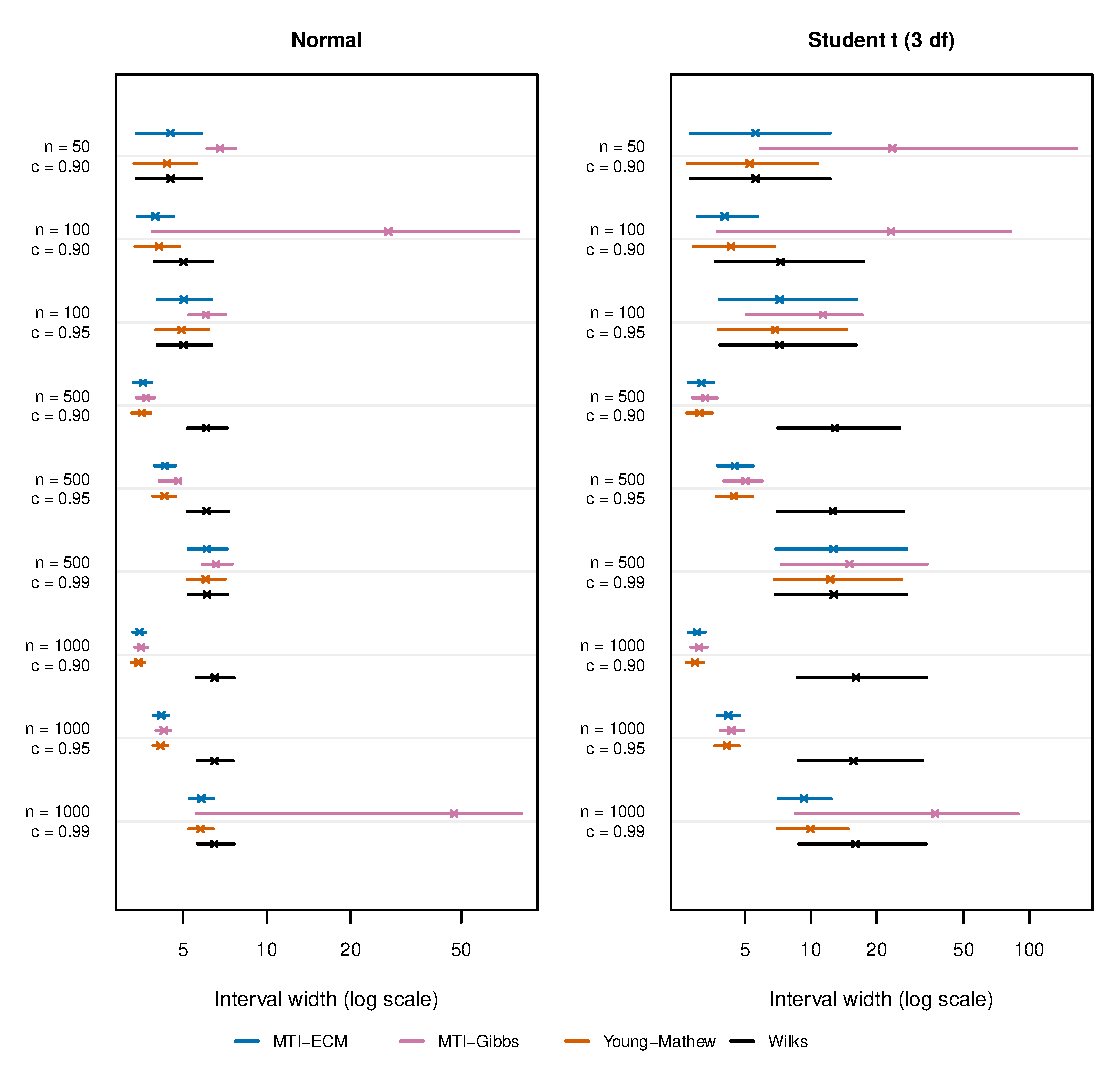
\includegraphics[width=\textwidth]{figures/generated/figS_mti_full_width_ranges_01.pdf}
\caption{\textbf{Raw width ranges for the two symmetric simulation laws.}
Segments give empirical 2.5\%--97.5\% quantiles across the 1000 samples
for each distribution, design, and method; crosses mark mean widths.
The horizontal axes are logarithmic, with values in response units.
The four intervals in each design group are separated from neighboring
designs. MTI-Gibbs uses posterior-mean endpoints.}
\label{fig:supp-mti-full-widths-symmetric}
\end{figure}

\begin{figure}[p]
\centering
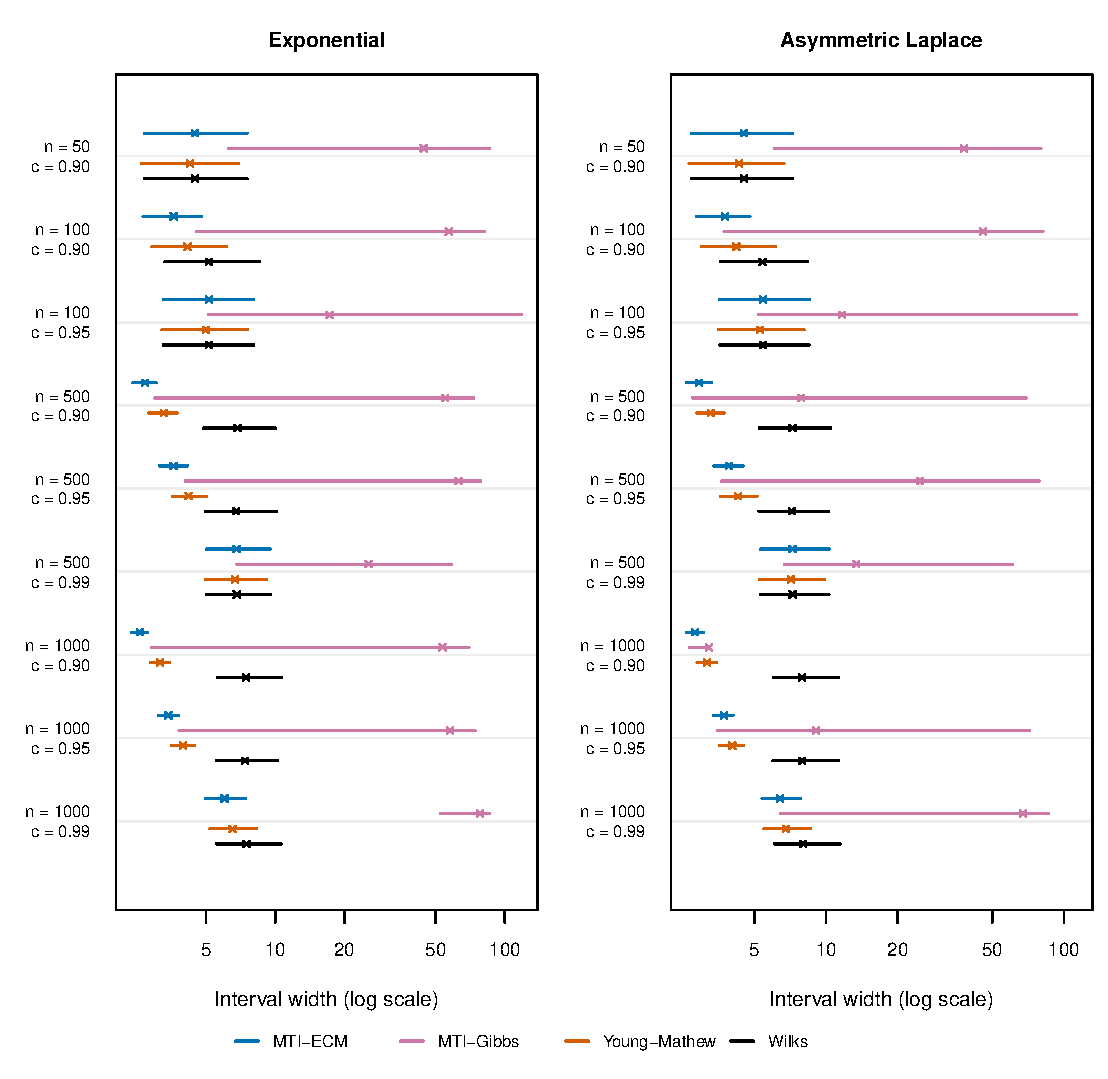
\includegraphics[width=\textwidth]{figures/generated/figS_mti_full_width_ranges_02.pdf}
\caption{\textbf{Raw width ranges for exponential and asymmetric Laplace samples.}
Segments, crosses, design grouping, and logarithmic axes follow
Figure~\ref{fig:supp-mti-full-widths-symmetric}. Each width range is
computed within its own distribution and design.}
\label{fig:supp-mti-full-widths-exponential-al}
\end{figure}

\begin{figure}[p]
\centering
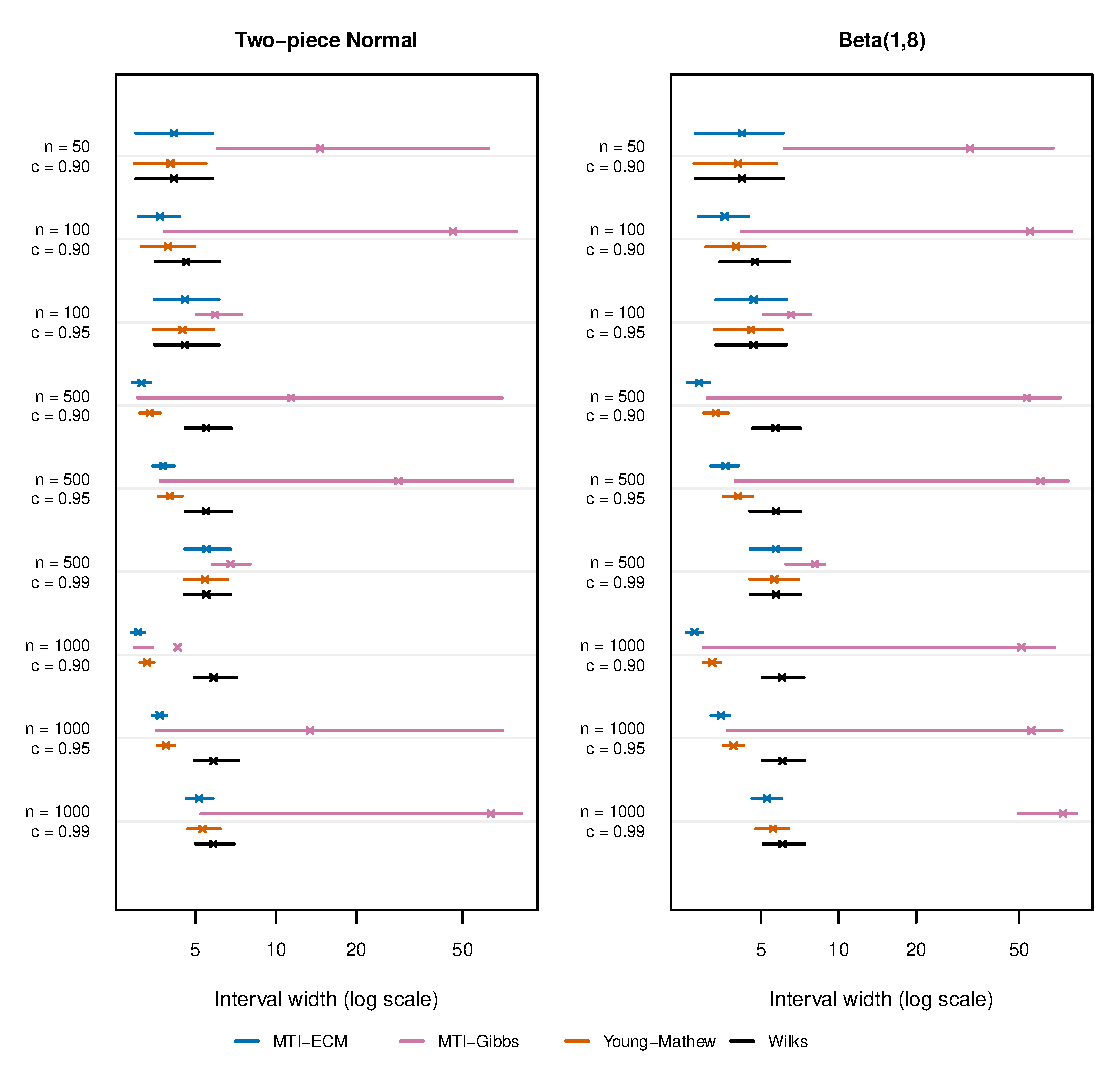
\includegraphics[width=\textwidth]{figures/generated/figS_mti_full_width_ranges_03.pdf}
\caption{\textbf{Raw width ranges for two-piece Normal and Beta samples.}
Segments, crosses, design grouping, and logarithmic axes follow
Figure~\ref{fig:supp-mti-full-widths-symmetric}. Wider posterior-mean
intervals remain visible on the original response scale.}
\label{fig:supp-mti-full-widths-two-piece-beta}
\end{figure}

\begin{figure}[p]
\centering
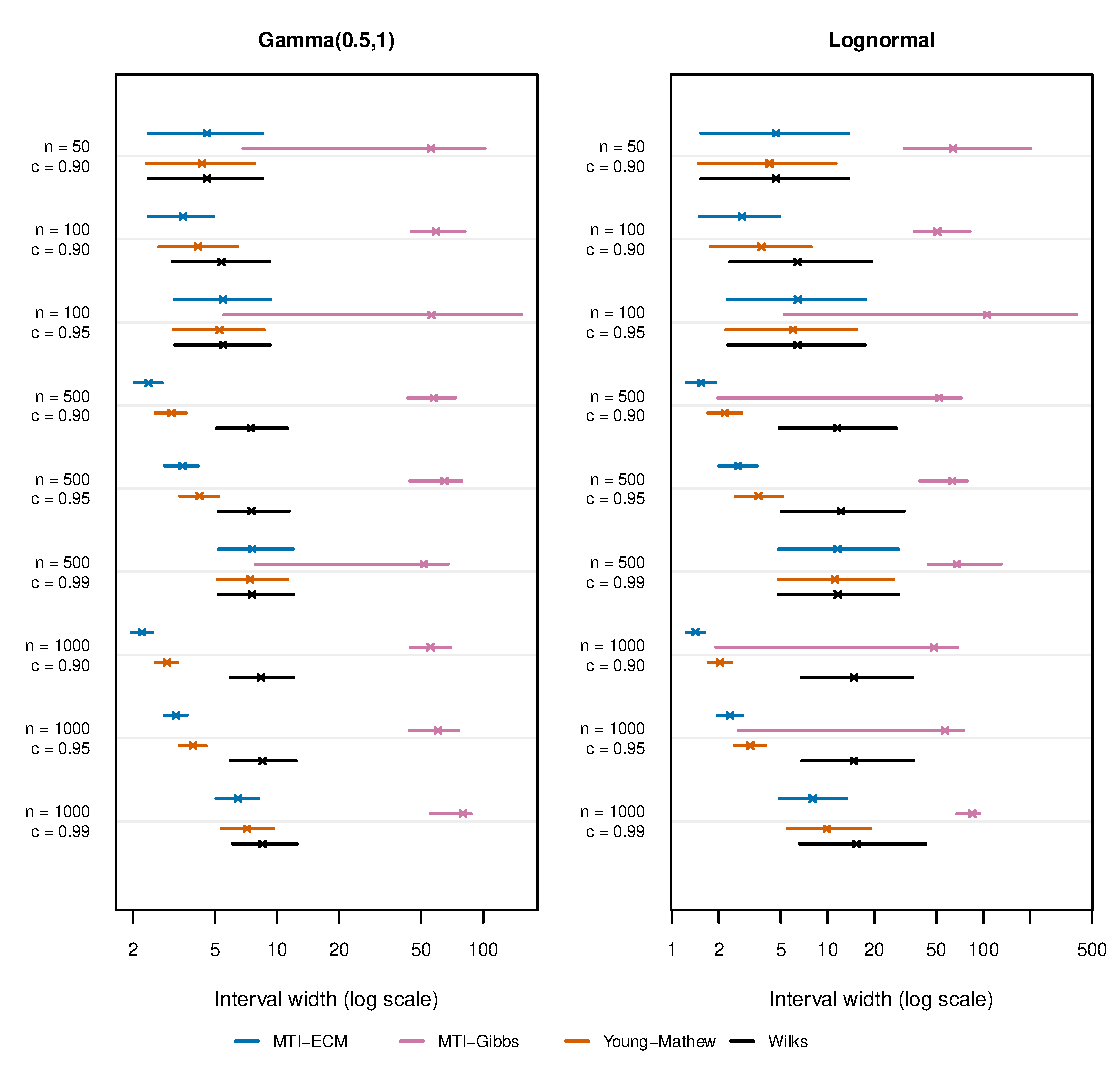
\includegraphics[width=\textwidth]{figures/generated/figS_mti_full_width_ranges_04.pdf}
\caption{\textbf{Raw width ranges for Gamma and lognormal samples.}
Segments, crosses, design grouping, and logarithmic axes follow
Figure~\ref{fig:supp-mti-full-widths-symmetric}. The larger Gibbs width
ranges accompany the empirical limiting-tilt behavior discussed in
Section~\ref{sec:supp-mti-posterior-assessment}.}
\label{fig:supp-mti-full-widths-gamma-lognormal}
\end{figure}
\clearpage
